\section{Neural networks}
Modern machine learning owes much of its popularity to the success of artificial neural networks, or if the context is clear, just neural networks (NNs).
With easier access to larger datasets, more powerful hardware (in particular GPUs or even dedicated TPUs) and the backpropagation algorithm, NNs have become able to solve problems far too complicated for traditional methods.

Though state-of-the neural networks can contain billions of parameters, training them remains feasible.
Modern hardware is of course paramount, but also backpropagation is crucial.
Neural networks are trained using gradient methods, and with backpropagation, the gradient can be computed efficiently.

With the great size and complexity, interpretability is sacrificed.
The models are often black boxes; it is difficult to understand why they make the predictions they do.
Luckily, there have been some developments, perhaps most notably the universal approximation theorem.
It states that a neural network with a single hidden layer can approximate any continuous function to arbitrary precision, given enough neurons\footnote{In addition to some requirements regarding the activation function.}.
This gives some credence to the idea that NNs of other structures could be used to approximate intricate functions.


\subsection{Architectures}
\subsubsection{Dense feed-forward neural networks}
The basic neural network is a dense feed-forward neural network, with a typical structure shown in \cref{fig:nn}.
There can be more or fewer nodes in each layer, and as many or few hidden layers as desired.

\begin{figure}
    \centering
    \includegraphics[width=0.7\linewidth, page=4]{neural_networks.pdf}
    \caption{
        Typical structure of a dense feed-forward neural network.
        Here it has three hidden layers of constant size $m$, but the number of layers and the size of each layer can be chosen arbitrarily.
        Being dense means that each node in one layer is connected to all nodes in the next layer, while being feed-forward means that the connections are unidirectional.
        From \cite{nn_figs}.
    }
    \label{fig:nn}
\end{figure}

In the input layer, the data is fed in with each input node corresponding to a feature.
Then, in the hidden layers, the data is transformed by a series of linear transformations and non-linear activation functions.
These can be expressed as
\begin{equation}
    \label{eq:nn}
    a_i^{(j)} = \sigma\left( \sum_{n=1}^m w^{(j)}_n a^{(j-1)}_n + b^{(j)}_n \right),
\end{equation}
where $j$ is the layer number, $i$ is the node number and $w$ and $b$ are the weights and biases of the network — parameters to be optimised.
The activation function $\sigma$ is a non-linear function, such as the sigmoid function, the hyperbolic tangent or the rectified linear unit (ReLU)
\begin{equation}
    \sigma(x) = \begin{cases}
        \frac{1}{1 + e^{-x}} & \text{sigmoid}            \\
        \tanh(x)             & \text{hyperbolic tangent} \\
        \max(0, x)           & \text{ReLU}
    \end{cases}
\end{equation}
which is needed for the model not to simply be a linear transformation.
The output layer is similar to the hidden layers, though perhaps with different activation functions and fewer nodes.
For instance, if the goal is to classify the data into $k$ classes, the output layer could have $k$ nodes with an activation function that ensures the sum of the outputs is one.
In that way, the output can be interpreted as probabilities.

A model like this is dense, because each node in one layer depends on every node in the previous layer.
It is feed-forward, because the data flows in one direction; the perceptrons in a layer depends only on those in the former.



\subsubsection{Convolutional neural networks}
Convolutional neural networks (CNNs) are a special type of neural network that are particularly suited for certain tasks like image processing.
A greatly simplified CNN is shown in \cref{fig:cnn}.

\begin{figure}
    \centering
    \includegraphics[width=0.75\linewidth, page=7]{neural_networks.pdf}
    \caption{
        The basic structure of a convolutional neural network.
        Data is input before conventional layers are applied, in which perceptrons are only connected to small regions of the previous layer.
        After sufficient dimensionality reduction, regular dense layers can be used.
        From \cite{nn_figs}.
    }
    \label{fig:cnn}
\end{figure}

The basic component of the CNN is the convolutional layer.
In it, a kernel or filter is applied to the input data, which often is as simple as a $3 \times 3$ matrix.
It is applied to only parts of the input, and thus only extracts local properties.
Typically, pooling layers complement the convolutions by reducing the dimensionality through some simple non-parametrised operation, such as taking the maximum value in a $2 \times 2$ matrix.
CNNs generally finish with one or more dense layers, which then operate on a significantly reduced number of features.
The reduction of dimensionality is important because it reduces the number of parameters in the model and the risk of overfitting.
Furthermore, the convolutional approach forces the model to learn local features.
This is very beneficial for tasks such as image classification, where local features, such as edges, are more important than global ones, such as the position of the subject.